\subsection{Caesar Cipher}
	
	The Caesar cipher is another substitution cipher named after the Julius Caesar, who used it to encrypt messages of military significance.
	
	This cipher is similar to Atbash, but instead of reversing the alphabet, the substitute alphabet is created by shifting letters.
	
	\begin{figure}[h]
		\centering
		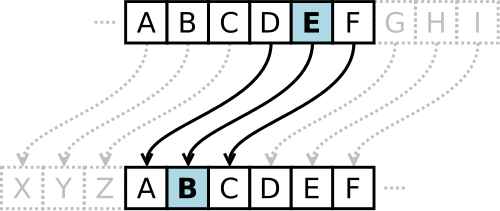
\includegraphics[width=0.5\linewidth]{McrRaspJam/016_Ciphers/2_caesar/caesarshift}
		\caption{Shifting letters to create the substitute alphabet}
		\label{fig:caesardiagram}
	\end{figure}
	
	\subsubsection{An Example}
	
		If we wish to encrypt the plaintext ``\textbf{The enemy surrounds us}'' with a rightward shift of \textbf{1} place, we can use the table in \autoref{fig:caeser} as follows:
		
		\begin{tabular}{ccccccc}
			T & $\rightarrow$ & u && e & $\rightarrow$ & f \\ 
			h & $\rightarrow$ & i && n & $\rightarrow$ & o \\ 
			e & $\rightarrow$ & f && e & $\rightarrow$ & f\\ 
			 & & && m & $\rightarrow$ & n\\ 
			 & & && y & $\rightarrow$ & z\\
		\end{tabular}
	
		Our full ciphertext for this phrase would be ``\mbox{\textbf{Uif fofnz tvsspvoet vt}}''.
		
		Returning to your pen and paper, have a go at encoding the following phrase.
		
		``\textbf{Attack from the west}'', right shift of \textbf{3}.
		
		Then try the following. You will need to construct your own substitute alphabet for this:
		
		``\textbf{The city has fallen}'', \textit{left} shift of \textbf{2}.
		
		\begin{figure*}
			\begin{tabular}{r|cccccccccccccccccccccccccc}
				\textbf{plaintext} & a & b & c & d & e & f & g & h & i & j & k & l & m & n & o & p & q & r & s & t & u & v & w & x & y & z \\ 
				\hline
				\textbf{Right 1} & b & c & d & e & f & g & h & i & j & k & l & m & n & o & p & q & r & s & t & u & v & w & x & y & z & a\\
				\textbf{Right 2} & c & d & e & f & g & h & i & j & k & l & m & n & o & p & q & r & s & t & u & v & w & x & y & z & a & b\\
				\textbf{Right 3} & d & e & f & g & h & i & j & k & l & m & n & o & p & q & r & s & t & u & v & w & x & y & z & a & b & c\\
			\end{tabular} 
			\caption{Caesar shift substitutions for the first three values of right shift}
			\label{fig:caeser}
		\end{figure*}

	\subsubsection*{Caesar Cipher in Python}
	
		Because the Caesar cipher is so similar to Atbash, we can reuse most of the code from that program.
		
		\textbf{Copy} the Atbash program---either through the file manager, or by \texttt{File $\rightarrow$ Save As...}---and rename, then open the new file.
		
		The first addition we will add to our program will be to allow the user to determine the shift for the cipher. We can do this with another \texttt{input()} function.
		
		\lstinputlisting[style=Python, title=caesar.py, firstline=3, firstnumber=3, lastline=6, breaklines=true]{McrRaspJam/016_Ciphers/2_caesar/caesar.py}
		
		Then, we need to create the substitute alphabet based on the shift number. This is more complex than Atbash, so we'll start with an empty list, and fill it using a loop.
		
		\lstinputlisting[style=Python, firstline=7, firstnumber=7, lastline=9]{McrRaspJam/016_Ciphers/2_caesar/caesar.py}
		
		To shift the letters, we'll first get the ASCII code for the letter and subtract 97, just like we did last time:
		
		\lstinputlisting[style=Python, firstline=10, firstnumber=10, lastline=13]{McrRaspJam/016_Ciphers/2_caesar/caesar.py}
		
		then we'll add the shift number. To wrap from one end of the alphabet to the other, we'll use a \textit{modulus} operator.
		
		\lstinputlisting[style=Python, firstline=14, firstnumber=14, lastline=14]{McrRaspJam/016_Ciphers/2_caesar/caesar.py}

		\ifprint\else
			\begin{aside}[Modulus Operation]
				The modulus operation (signified by \texttt{\%}) finds the remainder of a division.
				
				For the letter `x' (23)
				
				\begin{align*}
					23 \div 26 &= 0 \text{ remainder } \textbf{23}
				\end{align*}
				
				When shifted by 5, it `wraps around' to the start of the alphabet :
				
				\begin{align*}
					28 \div 26 &= 1 \text{ remainder } \textbf{2}
				\end{align*}
				
			\end{aside}
		\fi
		
		Finally, we grab the letter at this place in the alphabet, and add that to our substitute alphabet
		
		\lstinputlisting[style=Python, firstline=15, firstnumber=15, lastline=15, breaklines=true]{McrRaspJam/016_Ciphers/2_caesar/caesar.py}
		
		Your program should now be complete. Try encoding the phrases from the pen and paper examples, and see if they match.
		
		Have a think about the same questions we asked after we finished the Atbash program.
		
		\ifprint\else
			\begin{itemize}[nosep]
				\item Our program currently \textit{encodes} Caesar ciphers. What would we have to do to write a decoding program?
				\item What makes the Caesar cipher more secure than Atbash?
			\end{itemize}
		\fi

	\subsubsection*{Cryptographic Key}
	
		When we introduce a variable into an encryption method, we call this a cryptographic \textbf{key}. (sometimes called a \textit{cryptovariable})
		
		In Atbash, there is only one way that the alphabet is arranged, so there is no key. In the Caesar cipher, the cipher can be varied each time the cipher is used, so the shift number is the key for this cipher.
		
		\ifprint\else By introducing a key, an encrypted message can stay secure even if an intercepting party knows what cipher was used. However, the key \textit{must} be kept secret to maintain the security of the ciphertext. \fi

\subsection{Cracking the Caesar Cipher}

		If we don't hold the key to a ciphertext, we'll need to crack the code to access the plaintext.
		
		Because of the amazing computing speed of our Raspberry Pi, the easiest way to do this is to try every possible key in turn until we find the plaintext.
		
		\textbf{Open} the file \texttt{crackcaesar.py}, which contains a modified version of the program you just wrote.
		
		The program has been modified to use functions---which we will use shortly---and variable names have been switched to show that the program now goes from ciphertext to plaintext.
		
		The first modification we need is to make the decryption repeat to try each possible key. We'll place all of our previous code in a loop. (except for the input ciphertext)
		
		\lstinputlisting[style=Python, firstline=9, firstnumber=9, lastline=13, breaklines=true, title=crackcaesar.py]{McrRaspJam/016_Ciphers/2_caesar/crackcaesarb.py}
		
		We also need a way to tell when the solution has been found. To do this, we will check for the following suspect keywords: ``\textit{Attack}'', ``\textit{enemy}'', ``\textit{ally}'' and ``\textit{retreat}''.
		
		After generating each possible plaintext, we'll call the \texttt{check()} function. \textbf{Change} the following line:
	
		\begin{lstlisting}[style=Python, firstnumber=25]
print(plaintext)
		\end{lstlisting}
		
		to:
	
		\begin{lstlisting}[style=Python, firstnumber=25]
if check() == True:
	print(plaintext)
	break
		\end{lstlisting}
		
		The \texttt{check()} function will be very simple. It simply returns \texttt{True} if one of the words is found.
		
		\lstinputlisting[style=Python, firstline=28, firstnumber=28, lastline=30]{McrRaspJam/016_Ciphers/2_caesar/crackcaesara.py}
		
		Currently, the function always returns true, meaning the program always thinks it's found the solution on the first attempt.
		
		The following code returns true if the word ``attack'' is found in the possible plaintext. \textbf{Extend} the function to find the other 3 words.
		
		\begin{lstlisting}[style=Python, firstnumber=35]
def check():
	global plaintext
	found = False

	if "attack" in plaintext:
		found = True
		
	return found
		\end{lstlisting}
		
		Your program should now be complete. Try decoding the following ciphertexts:
		
		\begin{tabular}{c}
			``\textbf{jwljwslslgfuw}'' \\ 
			``\textbf{exxegoirvsyxi}''\\ 
			``\textbf{nbyyhygsulyxyzyunyx}''\\ 
			``\textbf{wjnsktwhjfqqdytxtzym}''\\
		\end{tabular} 
		